\documentclass[ucs, notheorems, handout]{beamer}

\usetheme[numbers,totalnumbers,compress, nologo]{Statmod}
\usefonttheme[onlymath]{serif}
\setbeamertemplate{navigation symbols}{}

\mode<handout> {
    \usepackage{pgfpages}
    \setbeameroption{show notes}
    \pgfpagesuselayout{2 on 1}[a4paper, border shrink=5mm]
    \setbeamercolor{note page}{bg=white}
    \setbeamercolor{note title}{bg=gray!10}
    \setbeamercolor{note date}{fg=gray!10}
}

\usepackage[utf8x]{inputenc}
\usepackage[T2A]{fontenc}
\usepackage[russian]{babel}
%\usepackage{tikz}
\usepackage{ragged2e}
%\usepackage{t-angles}
%\usepackage{slashbox}
\usepackage{hhline}
%new calligraphic font for subspaces 
\usepackage{euscript}
\newcommand{\cA}{\EuScript{A}}
\newcommand{\cB}{\EuScript{B}}
\newcommand{\cC}{\EuScript{C}}
\newcommand{\cD}{\EuScript{D}}
\newcommand{\cE}{\EuScript{E}}
\newcommand{\cF}{\EuScript{F}}
\newcommand{\cG}{\EuScript{G}}
\newcommand{\cH}{\EuScript{H}}
\newcommand{\cI}{\EuScript{I}}
\newcommand{\cJ}{\EuScript{J}}
\newcommand{\cK}{\EuScript{K}}
\newcommand{\cL}{\EuScript{L}}
\newcommand{\cM}{\EuScript{M}}
\newcommand{\cN}{\EuScript{N}}
\newcommand{\cO}{\EuScript{O}}
\newcommand{\cP}{\EuScript{P}}
\newcommand{\cQ}{\EuScript{Q}}
\newcommand{\cR}{\EuScript{R}}
\newcommand{\cS}{\EuScript{S}}
\newcommand{\cT}{\EuScript{T}}
\newcommand{\cU}{\EuScript{U}}
\newcommand{\cV}{\EuScript{V}}
\newcommand{\cW}{\EuScript{W}}
\newcommand{\cX}{\EuScript{X}}
\newcommand{\cY}{\EuScript{Y}}
\newcommand{\cZ}{\EuScript{Z}}

%font for text indices like transposition X^\mathrm{T}
\newcommand{\rmA}{\mathrm{A}}
\newcommand{\rmB}{\mathrm{B}}
\newcommand{\rmC}{\mathrm{C}}
\newcommand{\rmD}{\mathrm{D}}
\newcommand{\rmE}{\mathrm{E}}
\newcommand{\rmF}{\mathrm{F}}
\newcommand{\rmG}{\mathrm{G}}
\newcommand{\rmH}{\mathrm{H}}
\newcommand{\rmI}{\mathrm{I}}
\newcommand{\rmJ}{\mathrm{J}}
\newcommand{\rmK}{\mathrm{K}}
\newcommand{\rmL}{\mathrm{L}}
\newcommand{\rmM}{\mathrm{M}}
\newcommand{\rmN}{\mathrm{N}}
\newcommand{\rmO}{\mathrm{O}}
\newcommand{\rmP}{\mathrm{P}}
\newcommand{\rmQ}{\mathrm{Q}}
\newcommand{\rmR}{\mathrm{R}}
\newcommand{\rmS}{\mathrm{S}}
\newcommand{\rmT}{\mathrm{T}}
\newcommand{\rmU}{\mathrm{U}}
\newcommand{\rmV}{\mathrm{V}}
\newcommand{\rmW}{\mathrm{W}}
\newcommand{\rmX}{\mathrm{X}}
\newcommand{\rmY}{\mathrm{Y}}
\newcommand{\rmZ}{\mathrm{Z}}

%tt font for time series
\newcommand{\tA}{\mathsf{A}}
\newcommand{\tB}{\mathsf{B}}
\newcommand{\tC}{\mathsf{C}}
\newcommand{\tD}{\mathsf{D}}
\newcommand{\tE}{\mathsf{E}}
\newcommand{\tF}{\mathsf{F}}
\newcommand{\tG}{\mathsf{G}}
\newcommand{\tH}{\mathsf{H}}
\newcommand{\tI}{\mathsf{I}}
\newcommand{\tJ}{\mathsf{J}}
\newcommand{\tK}{\mathsf{K}}
\newcommand{\tL}{\mathsf{L}}
\newcommand{\tM}{\mathsf{M}}
\newcommand{\tN}{\mathsf{N}}
\newcommand{\tO}{\mathsf{O}}
\newcommand{\tP}{\mathsf{P}}
\newcommand{\tQ}{\mathsf{Q}}
\newcommand{\tR}{\mathsf{R}}
\newcommand{\tS}{\mathsf{S}}
\newcommand{\tT}{\mathsf{T}}
\newcommand{\tU}{\mathsf{U}}
\newcommand{\tV}{\mathsf{V}}
\newcommand{\tW}{\mathsf{W}}
\newcommand{\tX}{\mathsf{X}}
\newcommand{\tY}{\mathsf{Y}}
\newcommand{\tZ}{\mathsf{Z}}

%bf font for matrices
\newcommand{\bfA}{\mathbf{A}}
\newcommand{\bfB}{\mathbf{B}}
\newcommand{\bfC}{\mathbf{C}}
\newcommand{\bfD}{\mathbf{D}}
\newcommand{\bfE}{\mathbf{E}}
\newcommand{\bfF}{\mathbf{F}}
\newcommand{\bfG}{\mathbf{G}}
\newcommand{\bfH}{\mathbf{H}}
\newcommand{\bfI}{\mathbf{I}}
\newcommand{\bfJ}{\mathbf{J}}
\newcommand{\bfK}{\mathbf{K}}
\newcommand{\bfL}{\mathbf{L}}
\newcommand{\bfM}{\mathbf{M}}
\newcommand{\bfN}{\mathbf{N}}
\newcommand{\bfO}{\mathbf{O}}
\newcommand{\bfP}{\mathbf{P}}
\newcommand{\bfQ}{\mathbf{Q}}
\newcommand{\bfR}{\mathbf{R}}
\newcommand{\bfS}{\mathbf{S}}
\newcommand{\bfT}{\mathbf{T}}
\newcommand{\bfU}{\mathbf{U}}
\newcommand{\bfV}{\mathbf{V}}
\newcommand{\bfW}{\mathbf{W}}
\newcommand{\bfX}{\mathbf{X}}
\newcommand{\bfY}{\mathbf{Y}}
\newcommand{\bfZ}{\mathbf{Z}}

%bb font for standard spaces and expectation
\newcommand{\bbA}{\mathbb{A}}
\newcommand{\bbB}{\mathbb{B}}
\newcommand{\bbC}{\mathbb{C}}
\newcommand{\bbD}{\mathbb{D}}
\newcommand{\bbE}{\mathbb{E}}
\newcommand{\bbF}{\mathbb{F}}
\newcommand{\bbG}{\mathbb{G}}
\newcommand{\bbH}{\mathbb{H}}
\newcommand{\bbI}{\mathbb{I}}
\newcommand{\bbJ}{\mathbb{J}}
\newcommand{\bbK}{\mathbb{K}}
\newcommand{\bbL}{\mathbb{L}}
\newcommand{\bbM}{\mathbb{M}}
\newcommand{\bbN}{\mathbb{N}}
\newcommand{\bbO}{\mathbb{O}}
\newcommand{\bbP}{\mathbb{P}}
\newcommand{\bbQ}{\mathbb{Q}}
\newcommand{\bbR}{\mathbb{R}}
\newcommand{\bbS}{\mathbb{S}}
\newcommand{\bbT}{\mathbb{T}}
\newcommand{\bbU}{\mathbb{U}}
\newcommand{\bbV}{\mathbb{V}}
\newcommand{\bbW}{\mathbb{W}}
\newcommand{\bbX}{\mathbb{X}}
\newcommand{\bbY}{\mathbb{Y}}
\newcommand{\bbZ}{\mathbb{Z}}

%got font for any case
\newcommand{\gA}{\mathfrak{A}}
\newcommand{\gB}{\mathfrak{B}}
\newcommand{\gC}{\mathfrak{C}}
\newcommand{\gD}{\mathfrak{D}}
\newcommand{\gE}{\mathfrak{E}}
\newcommand{\gF}{\mathfrak{F}}
\newcommand{\gG}{\mathfrak{G}}
\newcommand{\gH}{\mathfrak{H}}
\newcommand{\gI}{\mathfrak{I}}
\newcommand{\gJ}{\mathfrak{J}}
\newcommand{\gK}{\mathfrak{K}}
\newcommand{\gL}{\mathfrak{L}}
\newcommand{\gM}{\mathfrak{M}}
\newcommand{\gN}{\mathfrak{N}}
\newcommand{\gO}{\mathfrak{O}}
\newcommand{\gP}{\mathfrak{P}}
\newcommand{\gQ}{\mathfrak{Q}}
\newcommand{\gR}{\mathfrak{R}}
\newcommand{\gS}{\mathfrak{S}}
\newcommand{\gT}{\mathfrak{T}}
\newcommand{\gU}{\mathfrak{U}}
\newcommand{\gV}{\mathfrak{V}}
\newcommand{\gW}{\mathfrak{W}}
\newcommand{\gX}{\mathfrak{X}}
\newcommand{\gY}{\mathfrak{Y}}
\newcommand{\gZ}{\mathfrak{Z}}

%old calligraphic font
\newcommand{\calA}{\mathcal{A}}
\newcommand{\calB}{\mathcal{B}}
\newcommand{\calC}{\mathcal{C}}
\newcommand{\calD}{\mathcal{D}}
\newcommand{\calE}{\mathcal{E}}
\newcommand{\calF}{\mathcal{F}}
\newcommand{\calG}{\mathcal{G}}
\newcommand{\calH}{\mathcal{H}}
\newcommand{\calI}{\mathcal{I}}
\newcommand{\calJ}{\mathcal{J}}
\newcommand{\calK}{\mathcal{K}}
\newcommand{\calL}{\mathcal{L}}
\newcommand{\calM}{\mathcal{M}}
\newcommand{\calN}{\mathcal{N}}
\newcommand{\calO}{\mathcal{O}}
\newcommand{\calP}{\mathcal{P}}
\newcommand{\calQ}{\mathcal{Q}}
\newcommand{\calR}{\mathcal{R}}
\newcommand{\calS}{\mathcal{S}}
\newcommand{\calT}{\mathcal{T}}
\newcommand{\calU}{\mathcal{U}}
\newcommand{\calV}{\mathcal{V}}
\newcommand{\calW}{\mathcal{W}}
\newcommand{\calX}{\mathcal{X}}
\newcommand{\calY}{\mathcal{Y}}
\newcommand{\calZ}{\mathcal{Z}}


\setbeamercolor{bluetext_color}{fg=blue}
\newcommand{\bluetext}[1]{{\usebeamercolor[fg]{bluetext_color}#1}}

\newtheorem{theorem}{Теорема}
\newtheorem{statement}{Утверждение}

\title[Tensor SSA]{Тензорный анализ сингулярного спектра}

\author{Хромов Никита Андреевич, гр.20.Б04-мм}

\institute[Санкт-Петербургский Государственный Университет]{%
    \small
    Санкт-Петербургский государственный университет\\
    Прикладная математика и информатика\\
    Вычислительная стохастика и статистические модели\\
    \vspace{1.25cm}
    Производственная практика (преддипломная практика)\\ (8 семестр)}

\date[Зачёт]{Санкт-Петербург, 2023}

\subject{Talks}

\begin{document}

    \begin{frame}[plain]
        \titlepage

        \note{Научный руководитель д.ф.-м.н., доцент Голяндина Н.Э.,\\
        кафедра статистического моделирования}
    \end{frame}


%\section{Короткая тема}
%\subsection{Общие слова}


    \section{Введение}\label{sec:intro}
    \begin{frame}{Постановка задачи}
        $\tX = (x_1, x_2, \ldots, x_N)$, $x_i \in \bbR$ --- вещественный временной ряд\\
        $\tX = \tT + \tP + \tR$\\
        $\tT$ --- тренд, $\tP$ --- сезонность, $\tR$ --- шум\\
        \vspace{0.3cm}
        
        \bluetext{Возможные задачи:}
        \begin{enumerate}
            \item Выделение сигнала из ряда: нахождение $\tS = \tT + \tP$
            \item Разделение компонент сигнала: нахождение $\tT$ и $\tP$
        \end{enumerate}
        \vspace{0.1cm}
        
        Возможный метод решения: Singular Spectrum Analysis (\bluetext{SSA})\\
        (Golyandina, Nekrutkin et al. (2001), Analysis of time series structure: SSA and related trchniques)\\
        \vspace{0.2cm}
        
        {\color{red} Цель:} исследованиге свойств тензорных модификаций методов семейства SSA с точки
        зрения точности выделения сигнала и разделения компонент.
        \note{
            Временным рядом длины N называется последовательность $N$ чисел. В общем случае, временной ряд является суммой трёх компонент: тренда $\tT$, сезонности $\tP$ и шума $\tR$.
            
            Можно рассматривать следующие задачи анализа временного ряда:
            
            Выделение сигнала $\tT+\tP$ из ряда,
            Отделение компонент сигнала $\tT$ и $\tP$.
            
            Одним из распространённых методов решения этих задач является алгоритм SSA, описанный в работе~\cite{ssa}.
            
            Цель этой работы - исследование свойств тензорных модификация методов семейства SSA с точки зрения точности выделения сигнала и отделения компонент сигнала.
        }
    \end{frame}
    
    \begin{frame}{Имеющиеся результаты}
        Работы, в котрых предлагается использовать тензорные разложения в задачах
        выделения сигнала из ряда:
        \begin{enumerate}
            \item Papy, De~Lathauwer et al. (2005), Exponential data fitting using
            multilinear algebra: the single-channel and multi-channel case
            \item Kouchaki, Sanei (2013), Tensor based singular spectrum analysis for
            nonstationary source separation
            \item Yang et al. (2017), Improved tensor-based Singular Spectrum Analysis
            based on single channel blind source separation algorithm and its application
            to fault diagnosis
        \end{enumerate}
        \vspace{0.2cm}
        
        В работе~1 рассматривается задача оценки параметров одномерных и многомерных
        сигналов особого вида с использованием тензорного разложения HOSVD.\\
        В работах 2 и 3 --- задача выделения сигнала из временного ряда с использованием
        тензорного разложения CPD.
        \note{
           На слайде представлены работы, в которых уже предлагалось использовать тензоры и тензорные разложения в задачах анализа временных рядов.
           
           В первой работе~\cite{tssa-hosvd} рассматривалась модель, в которой сигнал составляла сумма комплексных экспонент и нужно было оценить показатели их степеней. Для решения применялось тензорное разложение HOSVD, которое наследует большинство свойств матричного сингулярного разложения.
           
           Во второй и третьей работах рассматривалась задача выделения сигнала из зашумлённого ряда с применением тензороного разложения CPD. Подробнее про разложения далее.
           
           Пока был исследован только вариант перехода к тензорам, предложенный в первой работе.
        }
    \end{frame}
    
    \section{Тензорные модификации алгоритмов}
    \begin{frame}{ESPRIT}
        $\tX = (x_1, x_2, \ldots, x_N) = \tS + \tR$, $L$ -- длина окна,\\
        $K = N - L + 1 \geqslant L$.\\
        \vspace{0.1cm}
        
        \bluetext{Модель:} $s_n = \sum_{j=1}^{r} a_j \exp \{i \varphi_j\} 
        \exp \{(-\alpha_j + 2 \pi i \omega_j) n\}$\\
        \bluetext{Параметры алгоритма:} $L$, $R$: $R \leqslant L < N$\\
        $R$ --- число компонент, относимых к сигналу\\
        \vspace{0.1cm}
        
        \bluetext{Схема алгоритма ESPRIT для оценки $\alpha_j$, $\omega_j$}
        \begin{enumerate}
            \item \bluetext{Вложение} $\tX \mapsto \bfX = [X_1 : X_2 : \ldots : X_K] \in \bbR^{L \times K}$,\\
            $X_i = (x_i, x_{i+1}, \ldots, x_{i+L-1})^{\rmT}$
            \item \bluetext{Разложение} $\bfX = \sum_{j=1}^{d} \sqrt{\lambda_j}
            U_j V_j^{\rmT}$, $d \leqslant L$
            \item \bluetext{Группировка} $\widehat{\bfU} = [U_1: U_2: \ldots: U_R]$, $R\leqslant d$
            \item \bluetext{Восстановление} $\bfZ: \widehat{\bfU}^{\uparrow} = \widehat{\bfU}_{\downarrow}\bfZ$,\\
            $\{z_1, z_2, \ldots, z_R\}$ --- собственные числа $\bfZ$
        \end{enumerate}
        \bluetext{Результат алгоритма} $z_j$ --- оценка $\exp \{-\alpha_j + 2\pi i \omega\}$
        \note{
            \scriptsize
            В работе~\cite{tssa-hosvd} предлагалась модификация алгоритма ESPRIT для оценки параметров сигнала, равного сумме экспоненциально-модулированных комплексных гармоник.
            
            Пусть дан временной ряд $\tX$ длины $N$, и он является суммой некоторого сигнала $\tS$ и шума $\tR$. Выберем число $L$ - длина окна, и пусть она такова, что $K = N-K+1 \geqslant L$. Кроме того нужно выбрать параметр $R$, имеющий смысл числа компонент, которые мы относим к сигналу.
            
            Алгоритм состоит из следующих четырёх этапов:
            
            Вложение - по ряду $\tX$ строится матрица $\bfX$, $i$-й столбец которой представляет собой набор элементов ряда с $i$-го по $i+L-1$-й
            Разложение - матрица $\bfX$ представляется в виде своего сингулярного разложения в сумму $d$ одноранговых матриц
            Группировка - по первым $R$ левым сингулярным векторам строится матрица $\bfU$ с крышкой
            Восстановление - получившаяся на 3 шаге матрица $\bfU$ используется для решения уравнения, относительно $\bfZ$ (стрелка вверх означает удаление первой строки матрицы, стрелка вниз - последней). После этого находятся собственные числа полученной матрицы $\bfZ$, которые и считаются оценками экспонент, из которых можно получить оценки параметров.
        }
    \end{frame}
    
    \begin{frame}{SSA для выделения сигнала}
        $\tX = (x_1, x_2, \ldots, x_N) = \tS + \tR$, $L$ -- длина окна,\\
        $K = N - L + 1 \geqslant L$.\\
        \vspace{0.2cm}
        
        \bluetext{Параметры алгоритма:} $L$, $R$: $R \leqslant L < N$\\
        $R$ --- число компонент, относимых к сигналу\\
        \vspace{0.3cm}
        
        \bluetext{Схема алгоритма SSA для выделения сигнала}
        \begin{enumerate}
            \item \bluetext{Вложение} $\tX \mapsto \bfX = [X_1 : X_2 : \ldots : X_K] \in \bbR^{L \times K}$,\\
            $X_i = (x_i, x_{i+1}, \ldots, x_{i+L-1})^{\rmT}$
            \item \bluetext{Разложение} $\bfX = \sum_{j=1}^{d} \sqrt{\lambda_j}
            U_j V_j^{\rmT}$, $d \leqslant L$
            \item \bluetext{Группировка}  $\widetilde{\bfS} = \sum_{j=1}^{R} \sqrt{\lambda_j}
            U_j V_j^{\rmT}$, $R\leqslant d$
            \item \bluetext{Восстановление} Матрица $\widetilde{\bfS}$ усредняется вдоль побочных
            диагоналей: $\tilde{s}_k = \operatorname{mean}\left\{\left(\widetilde{\bfS}_{ij}\right)
            \middle| i + j - 1 = k\right\}$
        \end{enumerate}
        \bluetext{Результат алгоритма} $\widetilde{\tS} = (\tilde{s}_1, \tilde{s}_2, \ldots,
        \tilde{s}_N)$ --- оценка сигнала $\tS$
        \note{
            Теперь приведём алгоритм SSA для выделения сигнала.
            
            Пусть дан временной ряд $\tX$ длины $N$, и он является суммой некоторого (в этот раз непараметрического) сигнала $\tS$ и шума $\tR$. Параметры алгоритма и первые два его шага совпадают с алгоритмом ESPRIT.
            
            Группировка - по первым $R$ слагаемым из сингулярного разложения строится новая матрица $\widetilde{\bfS}$. Восстановление - получившаяся на 3 шаге матрица $\widetilde{\bfS}$ усредняется вдоль побочных диагоналей, результаты усреднения считаются результатом алгоритма.
        }
    \end{frame}
    
    \begin{frame}{Тензорный переход}
        Идея, предложенная в работе Papy et al. (2005)\\
        \vspace{0.3cm}
        
        \begin{table}
            \hspace*{-0.9cm}
            \begin{tabular}{rlllll}
                \bluetext{Базовый алгоритм:} & ряд $\tX$ & $\Rightarrow$ & матрица $\mathbf{X}$ & $\Rightarrow$ & SVD $\mathbf{X}$ \\
                \bluetext{Тензорный алгоритм:} & ряд $\tX$ & $\Rightarrow$ & тензор $\mathcal{X} $ & $\Rightarrow$ &
                \hspace*{-0.3cm} \begin{tabular}{l}
                    тензорное  \\
                    разложение
                \end{tabular} $\mathcal{X}$
            \end{tabular}
        \end{table}
        
        \vspace{0.4cm}
        Тензорные разложения, расширяющие SVD:
        \begin{itemize}
            \item High-order singular value decomposition (\bluetext{HOSVD})
            \item Canonical polyadic decomposition (CPD)
            \item ($L_r, L_r, 1)$-decomposition
        \end{itemize}
        
        \vspace{0.3cm} Их описание в обзорной работе Sidiropoulos, De~Lathauwer et al. (2016)

        \note{
            \scriptsize
            
            Как осуществить переход к тензорам? Если в SSA по ряду строится траекторная матрица, то в тензорном аналоге предлагается строить некоторый траекторный тензор, а сингулярное разложение предлагается заменить некоторым (аналогичным) тензорным разложением.
            
            В работе~\cite{tssa-hosvd} применяется разложение HOSVD (сингулярное разложение высшего порядка), однако существуют и другие тензорные разложения, которые расширяют сингулярное, CPD (каноническое полиадическое разложение) и $(L_r, L_r, 1)$-разложение.
            
            CPD заключается в том, чтобы представить тензор в сумму как можно меньшего числа внешних произведений векторов, а $(L_r, L_r, 1)$-разложение заключается в том, чтобы представить тензор в виде суммы как можно меньшего числа слагаемых, котоыре выглядят, как внешне произведение матрицы ранга $L_r$ на вектор.
            
            Про HOSVD более подробно будет рассказано позже.
            
            Описания этих и других тензорных разложений, а также примеры их применения в задачах обработки сигналов и машинного обучения, представлены в обзорной работе Sidiropoulus, De~Lathauwer et al. от 2016.\\
            Также выбор HOSVD можно обосновать тем, что оно среди всех разложений имеет наибольшее число свойств,
            схожих с обычным сингулярным разложением, и кроме того, другие разложения являются аппроксимациями или
            требуют предварительного знания некоторых параметров тензора.
        }
    \end{frame}


    \section{High-Order SSA}\label{sec:known}
    
    \begin{frame}{Описание HOSVD}
        Пусть имеется тензор $\mathcal{A}\in \mathbb{C}^{I_1\times I_2 \times \ldots \times I_M}$, тогда HOSVD $\mathcal{A}$:

        \begin{equation*}
                  \mathcal{A}=\sum_{i_1=1}^{I_1} \sum_{i_2=1}^{I_2}\ldots \sum_{i_M=1}^{I_M} \mathcal{Z}_{i_1 i_2 \ldots i_M}
                  U^{(1)}_{i_1} \circ U^{(2)}_{i_2} \circ \ldots\circ U^{(M)}_{i_M},
        \end{equation*}
        где
        \begin{itemize}
            \item $\mathbf{U}^{(n)}=\left[U^{(n)}_{1}: \ldots: U^{(n)}_{I_n}\right]$ --- унитарные матрицы;
            \smallskip
            \item Тензор $\mathcal{Z}\in\mathbb{C}^{I_1\times I_2 \times \ldots \times I_M}$ удовлетворяет свойствам
            \begin{enumerate}
                \item полная ортогональность:
                \[
                    \langle\mathcal Z_{i_n=\alpha},\mathcal Z_{i_n=\beta}\rangle=0 \qquad \alpha\ne\beta,
                \]
                \item упорядоченность:
                \begin{equation*}
                    \|\mathcal Z_{i_n=1}\|\geqslant\|\mathcal Z_{i_n=2}\| \geqslant \ldots \geqslant\|\mathcal Z_{i_n=I_n}\|.
                \end{equation*}
            \end{enumerate}
        \end{itemize}

        \note{
            Любой комплекснозначный тензор $\mathcal{A}$ размерности $I_1\times I_2 \times \ldots \times I_M$, может быть представлен
            в виде суммы тензоров ранга $1$, то есть внешних произведений векторов, как показано на слайде.
            $M$ называется количеством измерений тензора.
            Такое представление называется HOSVD тензора $\mathcal{A}$, векторы $U_i^{(n)}$ называют
            $i$-м сингулярным вектором тензора $\mathcal A$ по измерению $n$, нормы Фробениуса подтензора $\mathcal{Z}$ с
            фиксированным $n$-м индексом равным $i$ называют $i$-м сингулярным значением тензора $\mathcal{A}$
            по измерению $n$.

            Свойство полной ортогональности является аналогом свойства диагональности матрицы сингулярных значений в SVD,
            а свойство упорядоченности собственных значений вдоль каждого измерения --- аналог упорядоченности собственных значений.
        }
    \end{frame}

    \begin{frame}{Свойства HOSVD}
        Все свойства представлены в работе De Lathauwer et al. (2000)
        \begin{itemize}
            \item HOSVD --- единственное $M$-ортогональное разложение.
            \vspace{0.3cm}
            \item При $M=2$ HOSVD совпадает с SVD\@.
            \vspace{0.3cm}
            \item Пусть $\operatorname{rank}_n(\mathcal{A})$ --- размерность
            пространства векторов измерения $n$ тензора.
            Если в HOSVD тензора $\mathcal{A}$ $r_n$ --- наибольший индекс такой, что $\|\mathcal{Z}_{i_n=r_n}\|>0$,
            то $r_n=\operatorname{rank}_n(\mathcal{A})$.
            \vspace{0.3cm}
            \item
            \begin{gather*}
                \|\mathcal{A}\|^2=\sum_{i=1}^{R_1}\left( \sigma_i^{(1)} \right)^2=\sum_{i=1}^{R_2}\left( \sigma_i^{(2)} \right)^2
                =\ldots =\sum_{i=1}^{R_M}\left( \sigma_i^{(M)} \right)^2= \|\mathcal{Z}\|^2\\
                \sigma_{i}^{(n)}=\|\mathcal{Z}_{{i_n}=i}\|, \qquad R_n=\operatorname{rank}_n(\mathcal{A}).
            \end{gather*}
        \end{itemize}
        \note{
        \footnotesize
            \begin{enumerate}
                \item HOSVD является единственным $M$-ортогональным разложением тензора, и сингулярные значения и векторы
                определяются с точностью до унитарных преобразований.
                \item Результат применения HOSVD к тензору с двумя измерениями, т.е. матрице, совпадает
                с результатом применения SVD к этой же матрице, в точности до унитарных преобразований сингулярных векторов и
                матрицы сингулярных значений.
                \item $n$-рангом тензора $\mathcal{A}$ называется размерность векторного пространства, порождённого
                векторами измерения $n$ этого тензора.
                Обозначается $R_n=\operatorname{rank}_{n}(\mathcal{A})$.
                Если в HOSVD тензора $\mathcal{A}$ $r_n$ --- наибольший индекс такой, что $\|\mathcal{Z}_{i_n=r_n}\|>0$,
                то $r_n=\operatorname{rank}_n(\mathcal{A})$;
                $n$-ранги являются характеристикой тензора, аналогичной матричным рангам.
                Однако в тензорном случае, $n$-ранги могут различаться, поэтому для каждого измерения определяется своя характеристика.
                \item Квадрат нормы тензора совпадает с суммами квадратов сингулярных значений по каждому из измерений и совпадает
                с квадратом нормы тензора $\mathcal{Z}$ из разложения.
            \end{enumerate}
        }
    \end{frame}

    \begin{frame}{Свойства HOSVD}
        \begin{itemize}
            \item Векторы тензора $\mathcal{A}$ по измерению $n$ в содержат наибольшие вклады в направлении $U^{(n)}_1$,
            величина этого вклада равна $\sigma^{(n)^2}_1$.
            Следующий по величине вклад по измерению $n$ достигается в направлении $U^{(n)}_2$,
            перпендикулярном $U^{(n)}_1$, с величиной $\sigma^{(n)^2}_2$, и т.д.
            \vspace{0.4cm}
            \item Определим тензор $\hat{\mathcal{A}}$ обнулением наименьших сингулярных значений $\sigma_{I_{n}'+1}^{(n)},
            \sigma_{I_{n}'+2}^{(n)},\ldots, \sigma_{R_n}^{(n)}$, тогда
            \begin{equation*}
                \|\mathcal{A}-\hat{\mathcal{A}}\|^2\leqslant \sum_{i_1=I_{1}'+1}^{R_1}\left( \sigma_{i_1}^{(1)}\right)^2 +
                \ldots + \sum_{i_M=I_{M}'+1}^{R_M}\left( \sigma_{i_M}^{(M)}\right)^2.
            \end{equation*}
        \end{itemize}
        \note{
            \scriptsize
            \begin{enumerate}
                \item Векторы тензора $\mathcal{A}$ по измерению $n$ содержат наибольший вклад в направлении $U^{(n)}_1$,
                и вклад в этом направлении равен $\sigma^{(n)^2}_1$.
                Следующий по величине вклад по измерению $n$ достигается в направлении $U^{(n)}_2$,
                перпендикулярном $U{(n)}_1$, с величиной $\sigma^{(n)^2}_2$, и так далее.
                \item Пусть $R_n=\operatorname{rank}_n(\mathcal{A})$.
                Определим тензор $\hat{\mathcal{A}}$ отбрасыванием наименьших сингулярных значений $\sigma_{I_{n}'+1}^{(n)}, \sigma_{I_{n}'+2}^{(n)},\ldots, \sigma_{R_n}^{(n)}$
                для заданных значений $I_{n}'$, $n \in \overline{1:M}$, то есть заменяя нулями соответствующие части тензора $\mathcal{Z}$.
                Тогда квадрат нормы разности тензоров не превосходит суммы квадратов отброшенных сингулярных значений.
            \end{enumerate}
            Эти свойства являются эквивалентом высшего порядка связи между SVD матрицы и ее наилучшим приближением,
            в смысле наименьших квадратов, матрицей более низкого ранга.
            Однако для тензоров ситуация совершенно иная.
            Тензор, полученный усечением HOSVD в общем случае не является наилучшим приближением при заданных
            ограничениях на ранги измерений, но это приближение всё же можно считать достаточно точным.
        }
    \end{frame}


    \section{HOSVD SSA: выделение сигнала}\label{sec:tssa-intro}
    
    \begin{frame}{Построение тензора}
        \centering
        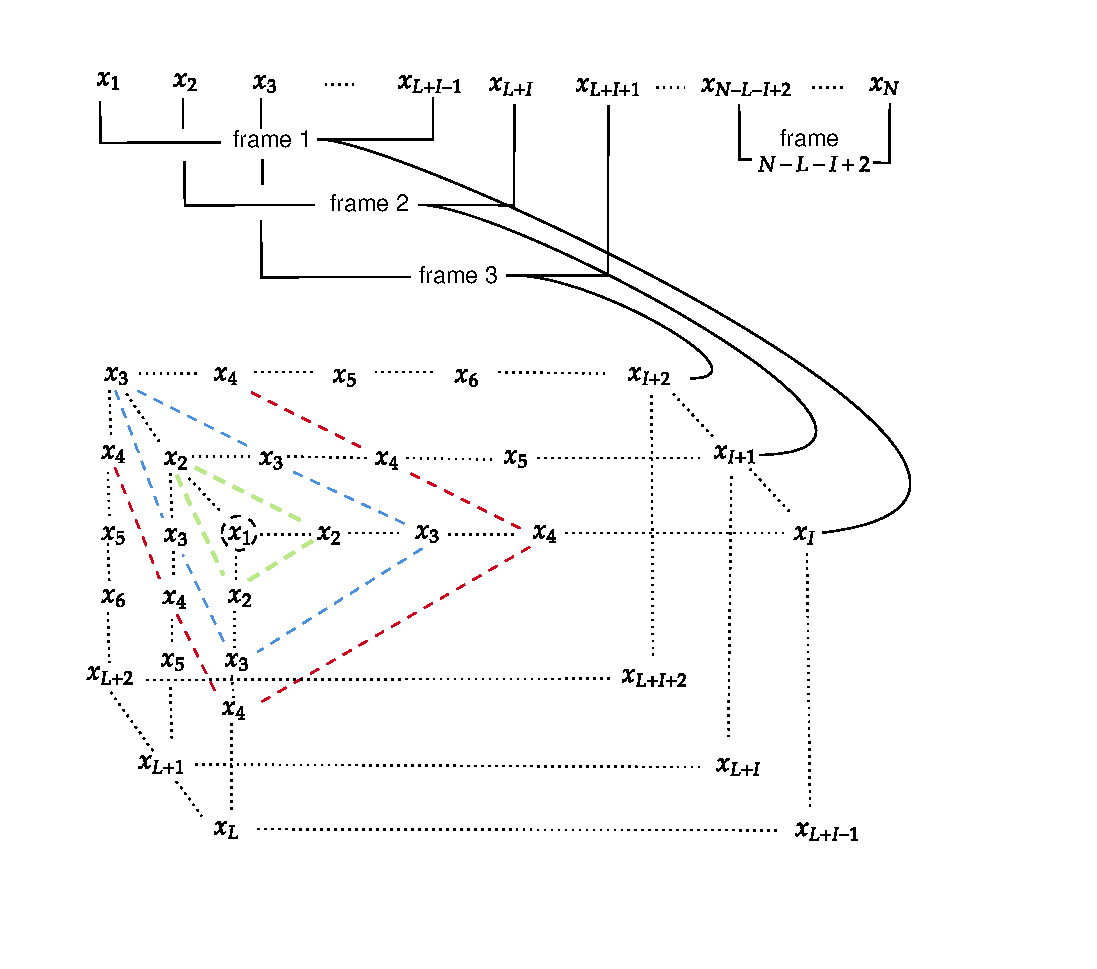
\includegraphics[width = \textwidth, height=0.8\textheight]{./img/tensor_injection_diagram}\\
        $I, L$ --- параметры длины окна
        \note{
            Теперь перейдём к описанию тензорных модификаций SSA, основные шаги которых были описаны в работе~\cite{tssa-hosvd}.
            
            Аналогично построению траекторной матрицы в алгоритме SSA, траекторный тензор строится следующим образом: сначала выбираются параметры $I$ и $L$, которые будем называть первой и второй длинами окна соответственно. Тогда $k$-й слой траекторного тензора вдоль 3-го измерения получается как траекторная матрица с длиной окна $L$, построенная по элементам ряда с $k$-го по $k+L+I-2$-й (визуализация представлена на слайде). При таком построении, получается, что на побочных диагоналях элементы совпадают (соединённые пунктирной линией одного цвета).\\
            Траекторный тензор будем обозначать символом X-красивое.
        }
    \end{frame}
    
    \begin{frame}{High-Order SSA для выделения сигнала}
        \begin{itemize}
            \item \bluetext{n-ранг тензора:} размерность пространства, порождённого векторами вдоль
            $n$-измерения тензора
            \item В отличие от матричного случая, $n$-ранги тензора произвольной размерности могут в общем случае
            не совпадать
        \end{itemize}
        
        \vspace{0.4cm}
        
        Основная идея алгоритма выделения сигнала --- приблизить траекторный тензор тензором с фиксированными
        $n$-рангами, меньшими, чем у исходного.
        \note{
            Напомним понятие $n$-ранга тензора: это размерность пространства, порождённого векторами вдоль $n$-го измерения тензора. Также вспомним, что в отличие от матричного случая, $n$-ранги тензора произвольной размерности могут в общем случае не совпадать.
            
            Основной идеей тензорной модификации алгоритма SSA для выделения сигнала является приближение траекторного тензора некоторым другим тензором с меньшими $n$-рангами.
        }
    \end{frame}
    
    \begin{frame}{HOSVD SSA: разложение и группировка}
        \begin{itemize}
            \item \bluetext{Разложение:} HOSVD траекторного тензора $\calX$ имеет вид
            \[
                \mathcal{X}=\sum_{i=1}^{I} \sum_{l=1}^{L} \sum_{j=1}^{N - I - L + 2} \mathcal{Z}_{ilj} \mathbf{U}^{(1)}_{i}
                \circ \mathbf{U}^{(2)}_{l} \circ \mathbf{U}^{(3)}_{j}
            \]
            
            \vspace{0.2cm}
            \item \bluetext{Группировка:}
            \[
                \widetilde{\calX} =\sum_{i=1}^{R} \sum_{l=1}^{R} \sum_{j=1}^{R} \mathcal{Z}_{ilj} \mathbf{U}^{(1)}_{i}
                \circ \mathbf{U}^{(2)}_{l} \circ \mathbf{U}^{(3)}_{j}
            \]
            $R \leqslant \min(I, L, N-I-L+2)$ --- параметр алгоритма
            
            \vspace{0.2cm}
            \item \bluetext{Восстановление:} усреднение тензора $\widetilde{\calX}$ вдоль побочных плоскостей
            $\left\{i + l + j = \operatorname{const}\right\}$
        \end{itemize}
        
        \note{
            Первая мысль --- урезать тензор сингулярных значений в HOSVD траекторного тензора по каждому измерению. В силу свойств HOSVD, такое усечение не даёт оптимальное приближение тезнора, но всё же оно довольно точное.
            
            На этапе разложения траекторный тензор предствляется в виде тройной суммы одноранговых тензоров.
            
            Этап группировки принимает вид обрезанной суммы, как представленно на слайде. У всех сумм один и тот же верхний предела в силу теоремы, которая будет сформулирована позже.
            
            Процесс восстановления является обратным к этапу вложения и заключается в усреднении элементов полученного тензора вдоль побочных гиперплоскостей (на которых сумма индексов - константа).
        }
    \end{frame}
    
    \section{HOOI SSA}
    \begin{frame}{Higher Order Orthogonal Iteration (HOOI)}
        Другой метод приближения произвольного тензора тензором заданных $n$-рангов --- Higher Order Orthogonal Iteration (HOOI).\\
        Описание алгоритма HOOI и его свойства приведены в работе Sheehan et al. (2007) Higher Order Orthogonal Iteration of Tensors (HOOI) and its Relation to PCA and GLRAM.\\
        При заданных $\calA \in \bbR^{I_1 \times I_2 \times \ldots \times I_M}$ и ($R_1, R_2, \ldots, R_M$)
        минимизируется норма Фробениуса 
        \[
            \| \calA - \widetilde{\calA}\|^2 \to \min,
        \]
        где $\min$ по всем $\widetilde{\calA}: \widetilde{\calA} \in \bbR^{I_1 \times I_2 \times \ldots \times I_M}$, 
        $\operatorname{rank}_n(\widetilde{\calA}) = R_i$
        
        \note{
            Другая мысль --- использовать метод ортогональных итераций высшего порядка HOOI, который по тензору и заданным n-рангам находит другой тензор этих n-рангов, наиболее точно приближающий исходный.
            
             Описание алгоритма HOOI и его свойства приведены в работе Sheehan et al. от 2007 г.
             
             При заданных $\calA \in \bbR^{I_1 \times I_2 \times \ldots \times I_M}$ и ($R_1, R_2, \ldots, R_M$)
             минимизируется норма Фробениуса 
             \[
                \| \calA - \widetilde{\calA}\|^2 \to \min,
             \]
             где $\min$ берётся по всем $\widetilde{\calA}: \widetilde{\calA} \in \bbR^{I_1 \times I_2 \times \ldots \times I_M}$, 
             $\operatorname{rank}_n(\widetilde{\calA}) = R_i$
        }
    \end{frame}
    
    \begin{frame}{HOOI SSA: разложение и восстановление}
        \begin{itemize}
            \item \bluetext{HOOI:} Выбор ранга сигнала $r$ и применение к траекторному тензору $\calX$ HOOI c 
            набором $n$-рангов $(r,r,r)$. Результат --- оптимальное приближение тензором $\widehat{\calX}$ с 
            $n$-рангами $r$
            \item \bluetext{Восстановление:} усреднение тензора $\widehat{\calX}$ аналогично восстановлению в 
            варианте с усечением HOSVD
        \end{itemize}
        \vspace*{0.4cm}
        
        \bluetext{Результат алгоритма:} полученный усреднением ряд $\widehat{\tX}$ --- оценка сигнала $\tS$
        \note{
            Алгоритм выделения сигнала из ряда с использованием HOOI будет выглядеть следующим образом: шаг вложения такой же, а вместо шага разложения к тензору применяется метод ортогональных итераций. Этап восстановления тот же, что и в предыдущем алгоритме, то есть усреднение по побочным гиперплоскостям.
        }
    \end{frame}
    
    \section{Свойства HO-SSA в задаче выделения сигнала}
    \begin{frame}{Ранг сигнала}
        $\tS$ имеет ранг $r$, если $r < N / 2$ и \\
        $\forall L: r \leqslant \min(L, K)\quad \operatorname{rank}\bfS = r$\\
        \vspace{0.2cm}
        
        Рекомендуемый выбор параметра $R$ в алгоритме: $R = r$\\
        \vspace{0.4cm}
        
        \bluetext{Примеры}
        \begin{enumerate}
            \item $s_n = \cos(2 \pi n \omega + \psi), \qquad n \in \overline{1:N}$,\\
            $0 < \omega < 1/2$, $\psi \in [0, 2\pi)$\\
            $r = 2$
            
            \vspace{0.2cm}
            
            \item $s_n = a^n,\qquad n \in \overline{1:N}, \qquad a \ne 0$\\
            $r =1$
        \end{enumerate}
        \note{
            Встаёт проблема выбора параметра $R$ в обоих алгоритмах.
            
            Важным понятием в теории SSA является понятие ранга ряда.
            
            Говорят, что сигнал $\tS$ имеет ранг $r$, если для любой длины окна $L: r \leqslant \min(L, K)$, ранг матрицы вложения $\bfS$, построенной по этой длине окна равен $r$.
            
            Это понятие позволяет свести выбор параметра $R$ из алгоритма к определению ранга сигнала, после чего $R$ рекомендуется выбирать равным $r$.
            
            Примеры:
            
            Функция косинуса с частотой $\omega$ и фазой $\psi$ при выполнении условий на частоту имеет ранг 2.
            
            Показательная функция имеет ранг 1.
        }
    \end{frame}
    
    \begin{frame}{Ранг в HOSVD SSA}
        \begin{theorem}
            Пусть сигнал $\tS$ имеет конечный ранг $r$ в терминах \emph{SSA}.\\
            Тогда для любых значений параметров $I$ и $L$ таких, что
            \[
                r \leqslant \min(I, L, N-I-L+2),
            \] 
            все $n$-ранги траекторного тензора $\calX$ этого сигнала с длинами окна $I$ и $L$ будут равны $r$.
        \end{theorem}
        \note{
            Мной было получено утверждение, позволяющее перенести понятие ранга сигнала из теории SSA на тензорный вариант: при выполнении некоторых условий, все $n$-ранги траекторного тензора $\calX$ будут равны рангу этого сигнала.
            
            Таким образом, выбор $R$ в тензорных алгоритмах аналогичен выбору $R$ в стандартном алгоритме SSA.
        }
    \end{frame}
    
    \begin{frame}{Трудоёмкость алгоритмов HO-SSA}
        \begin{itemize}
            \item \bluetext{HOSVD-SSA:} вычисление HOSVD тензора размерности $I\times L \times J$ имеет трудоёмкость порядка
            \[
                O(ILJ(\min(I, LJ) + \min(L, IJ) + \min(J, IL))).
            \]
            Если требуется вычислить только усечение HOSVD с $n$-рангами $(r_1, r_2, r_3)$, то трудоёмкость можно
            уменьшить до порядка
            \[
                O(ILJ(r_1 + r_2 + r_3)).
            \]
            \item \bluetext{HOOI-SSA:} HOOI --- итеративный алгоритм. Трудоёмкость каждой итерации имеет порядок
            \[
                O(r_1 r_2 r_3 (I + L + J)),
            \]
            а скорость сходимости алгоритма линейная.
        \end{itemize} 
        \note{
            \scriptsize 
            Рассмотрим трудоёмкость тензорных модификаций SSA. Так как шаг разложения является самым трудоёмким шагом в алгоритме HOSVD SSA, то для оценки трудоёмкости алгоритма достаточно оценить трудоёмкость сингулярного разложения траекторного тензора.
            
            Из известных свойств HOSVD и асимптотической трудоёмкости матричного SVD асимптотическая сложность HOSVD траекторного тензора, и всего алгоритма, имеет вид
            \[
                O(ILJ(\min(I, LJ) + \min(L, IJ) + \min(J, IL))).
            \]
            
            Если требуется найти только первые $r$ компонент SVD матрицы размерности $m\times n$, и $𝑟$ достаточно мало, то трудоёмкость можно уменьшить до $𝑂(rmn)$. Тогда эту модификацию можно применить для нахождения усечения HOSVD $n$-рангами $(r_1, r_2, r_3)$ и трудоёмкость составит 
            \[
                O(ILJ(r_1 + r_2 + r_3)).
            \]
            
            Оценим трудоёмкость алгоритма HOOI SSA. Самым трудоёмким шагом в алгоритме HOOI SSA является применение к траекторному тензору алгоритма ортогональных итераций. Этот алгоритм является итерационным, и известно, что в тех же обозначениях каждая итерация имеет асимптотическую сложность
            
            \[
                O(r_1 r_2 r_3 (I + L + J)),
            \]
            причём скорость сходимости алгоритма линейная.
        }
    \end{frame}
    
    \section{HOSVD-SSA: разделение компонент сигнала}
    \begin{frame}{HOSVD SSA: разделение компонент сигнала}
        Пусть $\tS = \sum_{k=1}^{m} \tS_k$\\
        Шаги вложения и разложения совпадают с алгоритмом HOSVD SSA для выделения сигнала.
         \begin{itemize}
            \item \bluetext{Группировка:} разбиение множества индексов $\mathfrak{S}=\{1,\, 2\,\ldots,\, \min(I, L, J)\}$ по смыслу на
            непересекающиеся множества $\mathfrak{S}_k,\, k\in\overline{1:m}$ и построение по этому разбиению тензоров
            \[
            \mathcal{X}^{(\mathfrak{S}_k)}=\sum_{i \in \mathfrak{S}_k} \sum_{l\in \mathfrak{S}_k} \sum_{j\in \mathfrak{S}_k}
            \mathcal{Z}_{ilj} \mathbf{U}^{(1)}_{i}\circ \mathbf{U}^{(2)}_{l} \circ \mathbf{U}^{(3)}_{j}.
            \]
            \item \bluetext{Восстановление:} получение рядов $\widetilde{\tS}_k$ по тензорам
            $\mathcal{X}^{(\mathfrak{S}_k)}$ посредством их усреднения вдоль плоскостей
             ${\{i+l+j=\operatorname{const}\}}$
        \end{itemize}
        
        \vspace{0.1cm}
        \bluetext{Результат алгоритма:} $\widetilde{\tS}_k$ --- оценка $\tS_k$.
        \note{
            Теперь приведём описание алгоритма HOSVD SSA для решения задачи отделения компонент сигнала. 
            Пусть сигнал $\tS$ является суммой сигналов $\tS_k$.
            Шаги вложения и разложения аналогичны тем, что были в алгоритме HOSVD SSA для выделения сигнала,
            поэтому описание продолжим с шага группировки. 
            На этом шаге множество индексов от одного до минимума по измерениям траекторного тензора разбивается пользователем на непересекающиеся множества $\gS_k$, и по каждому множеству строятся тензоры
            $\calX^{(\gS_k)}$ образом, как показано на слайде.
            
            Следующий шаг: восстановление, по каждому тензору $\calX^{(\gS_k)}$ восстанавливаются оценки рядов $\tS_k$ путём усреднения этих тензоров вдоль побочных гиперплоскостей. Результатом алгоритма будет набор оценок сигналов, составляющих исходный сигнал.
        }
    \end{frame}

    \begin{frame}{Разделимость рядов в HOSVD-SSA}
        \bluetext{Разделимость} рядов является важным понятием в теории SSA

        \vspace{0.5cm}
            \begin{theorem}
                Временные ряды $\widetilde{\tX}$ и $\widehat{\tX}$ длины $N$ слабо $I$- и
                $L$-разделимы в смысле теории \emph{SSA} тогда и только тогда, когда существует такое 
                \emph{HOSVD} траекторного тензора $\mathcal{X}$ ряда
                $\tX=\widetilde{\tX} + \widehat{\tX}$, что его можно в виде суммы \emph{HOSVD} траекторных тензоров рядов
                $\widetilde{\tX}$ и $\widehat{\tX}$.
            \end{theorem}

        \vspace{0.6cm}
        Понятие слабой разделимости рядов из SSA применимо к HO-SSA
        \note{
           Важную роль в теории SSA играет понятие разделимости. Мной было доказано следующее утверждение, позволяющее перенести понятие слабой разделимости из теории SSA на тензорный случай.
            
           Временные ряды $\widetilde{\tX}$ и $\widehat{\tX}$ длины $N$ слабо $I$- и
           $L$-разделимы в смысле теории SSA тогда и только тогда, когда существует такое 
           {HOSVD} траекторного тензора $\mathcal{X}$ ряда
           $\tX=\widetilde{\tX} + \widehat{\tX}$, что его можно в виде суммы {HOSVD} траекторных тензоров рядов
           $\widetilde{\tX}$ и $\widehat{\tX}$.
        }
    \end{frame}

   
   \section{HOSVD-MSSA}
   \begin{frame}{MSSA}
       \bluetext{Многомерный временной ряд:}\\
       $\tX = \left(\tX_1: \tX_2: \ldots: \tX_P\right), \qquad \tX_p = \left(x_1^{(p)}, x_2^{(p)}, \ldots, x_N^{(p)}\right)^{\rmT}$\\
       \vspace{0.2cm}
       
       \bluetext{Траекторная матрица этого ряда:}\\
       $\bfX = \left[\bfX_1 : \bfX_2 : \ldots : \bfX_P\right]$,\\
       $\bfX_p$ --- траекторная матрица $\tX_p$\\
       \vspace{0.2cm}
       
       Дальнейшие шаги алгоритма MSSA (разложение траекторной матрицы и восстановление сигнала) аналогичны
       стандартному SSA.\\
       \vspace{0.2cm}
       
       В случаях, когда сигналы $\tS_p$ имеют похожую структуру, использование MSSA даёт лучшие результаты, чем
       применение SSA к каждому ряду отдельно.
       
       \note{
            Теперь рассмотим расширение метода SSA для многомерных временных рядов: MSSA, причём будем рассматривать только задачу выделения сигнала. Под многомерным временным рядом будем понимать набор временных рядов одной длины. Траекторная матрица многомерного ряда с длиной окна $L$ строится стыковкой траекторных тензоров одномерных рядов с той же длиной окна по столбцам. Дальнейшие шаги MSSA (а именно: разложение траекторной матрицы и восстановление сигнала) аналогичны стандартному SSA для одномерных рядов.
            
            Стоит заметить, что из теории SSA известно, что в случаях, когда сигналы $\tS_{p}$ имеют похожую в некотором смысле структуру, использование MSSA даёт лучшие результаты, чем применение SSA к каждому ряду отдельно.
       }
   \end{frame}
   
   \begin{frame}{HOSVD-MSSA}
       Вместо матрицы $\bfX = \left[\bfX_1:\bfX_2 :\ldots: \bfX_P\right]$\\
       строится тензор $\calX: \calX_{\cdot \cdot p} = \bfX_p$
       
       \centering
       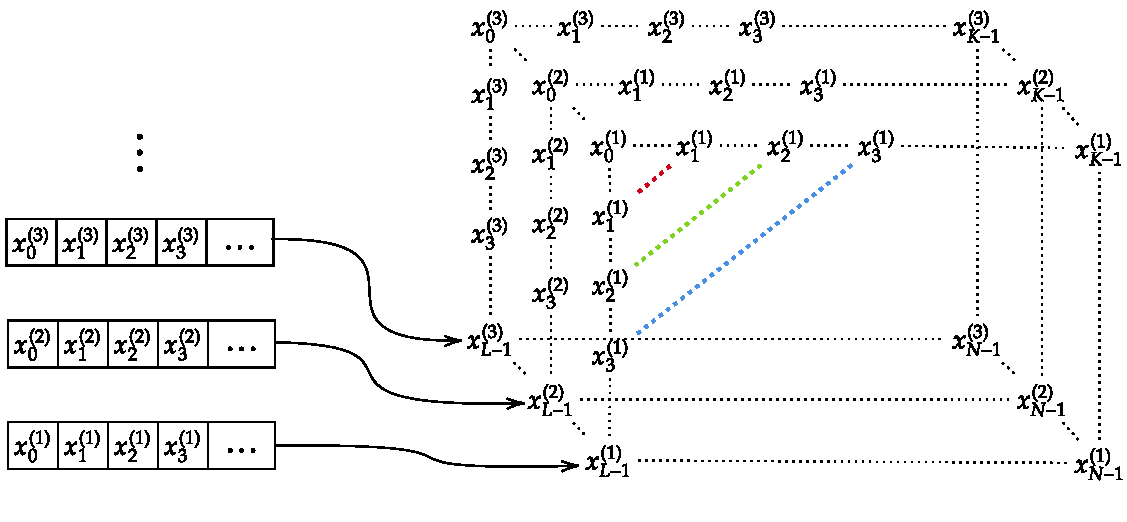
\includegraphics[width=\textwidth]{./img/mssa_injection}
       
       \note{
            В тензорной модификации вместо склеивания траекторных матриц по столбцам траекторный тензор строится склеиванием траекторных матриц рядов вдоль третьего измерения (<<накладыванием матриц в стопку>>). 
            Шаг разложения тот же, что и в алгоритме HOSVD SSA.
            
            Этап восстановления обратен этапу вложения.
        }
   \end{frame}
   
   \section{Свойства HOSVD-MSSA для выделения сигнала}
   \begin{frame}{Ранг сигнала в HOSVD-MSSA}
       
       \begin{theorem}
           Многомерный временной ряд 
           \[
                \left(x_0^{(p)}, x_1^{(p)}, \ldots, x_N^{(p)}\right), \quad p=1, 2, \ldots, P
           \]
           имеет ранг $r$ в терминах MSSA тогда и только тогда, когда для траекторного тензора 
           $\calX$, построенного по любой длине окна $L<N$ такой, что 
           $\min(L, K)\geqslant r$ выполняется $\operatorname{rank}_1(\calX) = \operatorname{rank}_2(\calX) = r$.\\
           Если к тому же $N > P$, то 3-ранг $\calX$ будет равен рангу матрицы, в строках которой содержатся
           одномерные временные ряды, составляющие заданный многомерный ряд.
       \end{theorem}
       
       \note{
           Мной было получено утверждение, позволяющее перенести понятие ранга ряда на тензорный вариант MSSA. 
           
           Многомерный временной ряд 
           \[
                \left(x_0^{(p)}, x_1^{(p)}, \ldots, x_N^{(p)}\right), \quad p=1, 2, \ldots, P
           \]
           имеет ранг $r$ в терминах MSSA тогда и только тогда, когда для траекторного тензора 
           $\calX$, построенного по любой длине окна $L<N$ такой, что 
           $\min(L, K)\geqslant r$ выполняется $\operatorname{rank}_1(\calX) = \operatorname{rank}_2(\calX) = r$.\\
           Если к тому же $N > P$, то 3-ранг $\calX$ будет равен рангу матрицы, в строках которой содержатся
           одномерные временные ряды, составляющие заданный многомерный ряд.
           
           Таким образом, исходя из этого утверждения, можно вывести рекомендации по выбору параметров $R_i$.
       }
   \end{frame}
   
   
   \begin{frame}{Ранг сигнала в HOSVD-MSSA}
       \begin{itemize}
           \item 1- и 2-ранги траекторного тензора $\calX$ сигнала $\tS$ совпадают с рангом этого сигнала в терминах
           MSSA
           \item 3-ранг имеет смысл степени структурного различия одномерных сигналов, составляющих данный многомерный
       \end{itemize}
       
       \vspace*{0.2cm}
       
       На этапе группировки рекомендуется брать $R_1=R_2=r$ и $R_3=r_3$, где $r$ --- MSSA-ранг сигнала, а 
       $r_3$ --- ранг матрицы, составленной из $\tS_p$\\
       \vspace{0.3cm}
       
       \bluetext{Примеры}
       $s_n^{(p)} = a_p \cos(2 \pi n \omega_p + \psi_p),\, p\in \{1, 2\},\, n \in \overline{1:N}$,\\
       $a_p \ne 0,\, 0 < \omega_p < 1/2,\, \psi_p \in [0, 2\pi)$
       \begin{enumerate}
           \item $\psi_1 = \psi_2,\, \omega_1 = \omega_2 \implies r = r_1 = r_2 = 2,\, r_3 = 1$ 
           \item $\psi_1 \ne \psi_2,\, \omega_1 = \omega_2 \implies r = r_1 = r_2 = 2,\, r_3 = 2$ 
           \item \hspace{42pt} $\omega_1 \ne \omega_2 \implies r = r_1 = r_2 = 4,\, r_3 = 2$ 
       \end{enumerate}
       
       \note{
           $R_1$ и $R_2$ рекомендуется выбирать равными рангу сигнала в терминах MSSA, а $R_3$ равным рангу матрицы, составленной из одномерных сигналов, составляющих данный многомерный сигнал.
           
           Этап группировки в алгоритме HO-MSSA рекомендуется проводить в соответствии с выбором параметров $R$ и $R3$.
           
           В качестве примера рассмотрим двумерный ряд, порождённый двумя косинусами.
           
           Если сигналы отличаются только домноженим на константу, то ранг сигнала в MSSA и его тензорном варианте равны 2, а ранг тензора вдоль третьего измерения равен 1.\\
           Если сигналы отличаются на сдвиг по фазе, то ранг сигнала всё ещё равен 2, но ранг тензора вдоль 3-го измерения уже будет 2.\\
           Если у синусов разные частоты, то ранг сигнала уже будет равен 4, а ранг $r_3$ -- 2.
       }
   \end{frame}
   
   \section{HO-MSSA: разделение компонент сигнала}
   \begin{frame}{HO-MSSA: разделение компонент сигнала}
       Пусть $\tS = \sum_{m=1}^{M} \tS_m$\\
       Шаги вложения и разложения совпадают с алгоритмом HO-MSSA для выделения сигнала
       
       \begin{itemize}
           \item \bluetext{Группировка} разбиение множества индексов ${\gS = \{1, 2, \ldots, \min(L, K)\}}$ и
           $\gP = \{1, 2, \ldots, P\}$ по смыслу
           на подмножества $\gS_m$ и $\gP_m$, $m \in \overline{1:M}$, и построение по этому разбиению 
           тензоров
           \[
                \calX_m = \sum_{l\in \gS_m} \sum_{k\in \gS_m} \sum_{p\in \gP_m}
                \calZ_{lkp} \bfU_l^{(1)} \circ \bfU_k^{(2)} \circ \bfU_p^{(3)} 
           \]
           \item \bluetext{Восстановление} получение рядов $\widetilde{\tS}_m$ по тензорам $\calX_m$ 
           путём усреднения их слоёв вдоль побочных диагоналей
       \end{itemize}
       
       \vspace{0.2cm}
       
       \bluetext{Результат алгоритма:} $\widetilde{\tS}_m$ --- оценка $\tS_m$
       
       \note{
           Наконец, приведём описание алгоритма HO-MSSA для отделения компонент сигнала.
           
           Шаги вложения и разложения совпадают с соответствующими шагами в алгоритме HO-MSSA для выделения сигнала.
           
           На этапе группировки строятся разбиения множества индексов $\gS$ и $\gP$ на подмножества
           $\gS_m$ и $\gP_m$, и по каждой паре этих множеств строятся тензоры $\calX_m$
           \[
                \calX_m = \sum_{l\in \gS_m} \sum_{k\in \gS_m} \sum_{p\in \gP_m}
                \calZ_{lkp} \bfU_l^{(1)} \circ \bfU_k^{(2)} \circ \bfU_p^{(3)} 
           \]
           
           Этап восстановления заключается в получении многомерных рядов $\widetilde{\tS}_m$ по тензорам $\calX_m$ аналогично шагу восстановления из алгоритма для выделения сигнала.
       }
   \end{frame}
   
   \begin{frame}{HO-MSSA: разделение компонент сигнала}
       $\widehat{\tX}$, $\widetilde{\tX}$, $\tX$ --- многомерные временные ряды, $\tX = \widehat{\tX} + \widetilde{\tX}$\\
       $\widehat{\calX}$, $\widetilde{\calX}$, $\calX$ --- траекторные тензоры рядов 
       $\widehat{\tX}$, $\widetilde{\tX}$, $\tX$ с длиной
       окна $L$\\
       $\Lambda_I(\tX) = \operatorname{span}\left\{(x_i^{(p)}, x_{i+1}^{(p)}, \ldots, x_{i + I - 1}^{(p)})\right\}$
       \begin{theorem}
           Такие HOSVD тензоров $\widehat{\tX}$ и $\widetilde{\tX}$, что их сумма является HOSVD тензора $\calX$ существуют
           тогда и только тогда, когда ортогональны пары пространств: \\
           $\Lambda_L(\widehat{\tX})$ с $\Lambda_L(\widetilde{\tX})$ и $\Lambda_K(\widehat{\tX})$ с
           $\Lambda_K(\widetilde{\tX})$
       \end{theorem}
       
       Этот критерий разделимости более строгий, чем в алгоритме MSSA\\
       \vspace{0.2cm}
       
       Этот критерий позволяет вывести рекомендации по выбору параметров $L$, $\gS_m$, $\gP_m$
       \note{
           Мной было получено утверждение, позволяющее выводить рекомендации по выбору параметров 
           $L$, $\gS_m$ и $\gP_m$ в алгоритме HO-MSSA для разделения компонент.
           
           Пусть $\widehat{\tX}$, $\widetilde{\tX}$, $\tX$ --- многомерные временные ряды ($\tX = \widehat{\tX} + \widetilde{\tX}$), \linebreak
           $\widehat{\calX}$, $\widetilde{\calX}$, $\calX$ --- траекторные тензоры рядов 
           $\widehat{\tX}$, $\widetilde{\tX}$, $\tX$ соответственно с длиной
           окна $L$.
           Обозначим 
           $\Lambda_I(\tX) = \operatorname{span}\left\{(x_i^{(p)}, x_{i+1}^{(p)}, \ldots, x_{i + I - 1}^{(p)})\right\}$.       
            
            \begin{theorem}
                Такие HOSVD тензоров $\widehat{\tX}$ и $\widetilde{\tX}$, что их сумма является HOSVD тензора $\calX$ существуют
                тогда и только тогда, когда ортогональны пары пространств: \\
                $\Lambda_L(\widehat{\tX})$ с $\Lambda_L(\widetilde{\tX})$ и $\Lambda_K(\widehat{\tX})$ с
                $\Lambda_K(\widetilde{\tX})$
            \end{theorem}    
            
            Стоит заметить, что этот критерий разделимости более строгий, чем в алгоритме MSSA.
       }
   \end{frame}
   
   
   \section{Численные сравнения}
   \begin{frame}{Численные сравнения: выделение сигнала}
       \begin{gather*}
           \tX = \left(\tX_1:\ldots : \tX_P\right),\\
           \tX_p = \left(s_1^{(p)} + \varepsilon_1^{(p)}, \ldots, s_N^{(p)} + \varepsilon_N^{(p)}\right),\\
           s_n^{(p)} = a_p \cos(2\pi n \omega_p + \psi_p),
       \end{gather*}
       где $n \in \overline{1:71}$, $p\in \overline{1:5}$, $\varepsilon_n^{(p)}$ --- белый гауссовский шум с дисперсией 25,
       $s_n^{(p)}$ --- элементы искомого сигнала.\\
       \vspace*{0.2cm}
       
       Оценка точности --- RMSE по 500 реализациям шума.
       
       \note{
           Было проведено два набора численных сравнений.
           
           Первый набор численных сравнений исследовал зависимость точности выделения сигнала в многомерных сигналах тензорных модификаций и известных методов семейства SSA. 
           Рассматриваемый сигнал имеет вид экспоненциально-модулированной гармоники, 
           шум -- белый гауссовский со стандартным отклонением 5. 
           Оценка точности производилась по RMSE по 500 реализациям шума. 
           Все методы сравнивались на одних и тех же реализациях шума.
           
           Было рассмотрено несколько вариантов значения $P$, приведём наиболее показательный случай, когда $P$=5.
       }
   \end{frame}
   
   \begin{frame}{Численные сравнения: ранги сигналов}
       
       \begin{table}
           \hspace*{-0.4cm}
           \footnotesize
           \begin{tabular}{c|cccc}
               Параметры & (HOOI) SSA & (HOSVD) MSSA & $r_3$ & 2D-SSA \\ \hline
               \begin{tabular}{c}
                   $a_p=30$\\
                   $\omega_p = 1/12,\, \psi_p = 0$
               \end{tabular} & 2 & 2 & 1 & 2 \\ \hline
               \begin{tabular}{c}
                   $a_1 = a_4 = 30$\\
                   $a_2=a_5=20$, $a_3 = 25$\\
                   $\omega_p = 1/12,\, \psi_p = 0$
               \end{tabular} & 2 & 2 & 1 & 6 \\ \hline
               \begin{tabular}{c}
                   $a_p=30$, $\omega_p=1/12$ \\
                   $\psi_p = 2(p-1)\pi / 3$
               \end{tabular} & 2 & 2 & 2 & 2 \\ \hline
               \begin{tabular}{c}
                   $a_p=30$, $\psi_p = 2(p-1)\pi / 3$\\
                   $\omega_1=\omega_2=\omega_3=1/12$ \\
                   $\omega_4=\omega_5=1/8$ 
               \end{tabular} & 2 & 4 & 4 & 10 \\ \hline
           \end{tabular}
       \end{table}
       
       \note{
           Для начала рассмотрим ранги сигналов для каждого метода при различных наборах параметров. 
           Меньше всего ранги во всех методах в случае, когда сигналы не отличаются между собой. 
           Когда сигналы отличаются только на амплитуду вырастает только 2D-SSA ранг. 
           Когда амплитуды и частоты сигналов равны, а частоты меняются линейно по p возрастает ранг третьего измерения в HOSVD MSSA. И наконец, когда амплитуды равны, фаза меняется линейно, а частоты разные, сильно возрастают ранги как HOSVD MSSA, так и 2D-SSA.
       }
   \end{frame}
   
   \begin{frame}{Численные сравнения: RMSE оценок сигналов}
       
       \begin{table}
           \hspace*{-0.6cm}
           \scriptsize
           \begin{tabular}{c|ccccc}
               Параметры & SSA & HOOI-SSA & MSSA & HOSVD-MSSA & 2D-SSA \\ \hline
               \begin{tabular}{c}
                   $a_p=30$\\
                   $\omega_p = 1/12,\, \psi_p = 0$
               \end{tabular} & 1.34 & 1.41 & 0.95 & 0.75 & \textbf{0.73} \\ \hline
               \begin{tabular}{c}
                   $a_1 = a_4 = 30$\\
                   $a_2=a_5=20$, $a_3 = 25$\\
                   $\omega_p = 1/12,\, \psi_p = 0$
               \end{tabular} & 1.38 & 1.41 & 1.07 & \textbf{0.86} & 1.45 \\ \hline
               \begin{tabular}{c}
                   $a_p=30$, $\omega_p=1/12$ \\
                   $\psi_p = 2(p-1)\pi / 3$
               \end{tabular} & 1.38 & 1.41 & 1.07 & 1.05 & \textbf{0.84} \\ \hline
               \begin{tabular}{c}
                   $a_p=30$, $\psi_p = 2(p-1)\pi / 3$\\
                   $\omega_1=\omega_2=\omega_3=1/12$ \\
                   $\omega_4=\omega_5=1/8$ 
               \end{tabular} & \textbf{1.38} & 1.41 & 1.50 & 1.49 & 1.78 \\ \hline
           \end{tabular}
       \end{table}
       
       \note{
           Теперь рассмотрим точность выделения сигнала каждым методом. Различия между всеми значениями в каждой строке значимы с уровнем значимости 0.05. Видно, что метод HOSVD MSSA работает лучше остальных методов в случае, когда сигналы отличаются только амплитудой, причём он всегда даёт более точные результаты, чем стандартный MSSA. В случае же когда сигналы отличаются и по фазе, и по частоте, самым точным оказывается применение SSA по отдельности к каждому ряду. 
           HO-SSA во всех сравнениях проигрывает стандартному SSA.
       }
   \end{frame}
   
   \begin{frame}{Численные сравнения: разделимость многомерных рядов}
       \[
            x_n^{(p)} = \hat{s}_n^{(p)} + \tilde{s}_n^{(p)} + \varepsilon_n^{(p)}
       \]
       \vspace*{0.1cm}
       
       $n \in \overline{1:44}$, $p \in \overline{1:12}$
       
       Рассматриваемые варианты рядов:
       \begin{enumerate}
           \item $\hat{s}_n^{(p)} = 2 \cos(2 \pi n / 5), \quad \tilde{s}_n^{(p)} = \cos(2\pi n /3)$
           
           \vspace{0.1cm}
           
           \item $\hat{s}_n^{(p)} = 2 c_1^{(p)} \cos(2 \pi n / 5), \quad \tilde{s}_n^{(p)} = c_2^{(p)}\cos(2\pi n /3)$
           
           \vspace{0.1cm}
           
           \item $\hat{s}_n^{(p)} = 2 c_1^{(p)} \cos(2 \pi n / 5 + p \pi / 6)$, \\
           $\tilde{s}_n^{(p)} = c_2^{(p)}\cos(2\pi n /3 + p \pi / 9)$
           
           \vspace{0.1cm}
           
           \item $\hat{s}_n^{(p)} = 2 c_1^{(p)} \cos(2 \pi n / 5 + \varphi_1^{(p)})$,\\ 
           $\tilde{s}_n^{(p)} = c_2^{(p)}\cos(2\pi n /3 + \varphi_2^{(p)})$
       \end{enumerate}
       
       \note{
           Второй набор численных сравнений исследовал точность отделения компонент в многомерных рядах методом HO-MSSA. 
           Все ряды имели вид суммы двух сигналов $\hat{s}_n^{(p)}$ и $\tilde{s}_n^{(p)}$ и белого гауссовского шума со стандартным отклонением 0.1.
           
           Были рассмотрены следующие варианты пар сигналов:
           
           \begin{enumerate}
               \item Оба сигнала полностью совпадали во всех каналах
               \item Сигналы отличались по каналам только амплитудой (далее все сигналы будут отличатся амплитудой по каналам, кроме случая 6)
               \item Линейно меняющаяся с номером канала фаза
               \item  У сигналов фазы отличаются во всех каналах случайным образом
           \end{enumerate}
       }
   \end{frame}
   
   \begin{frame}{Численные сравнения: разделимость многомерных рядов}
       
       \begin{enumerate}
           \setcounter{enumi}{4}
            \item $\hat{s}_n^{(p)} = 3 c_1^{(p)}, 
           \quad \tilde{s}_n^{(p)} = c_2^{(p)}\cos(2\pi n /3)$
           
           \vspace{0.2cm}
           
           \item $\hat{s}_n^{(p)} = 2 \cos(2 \pi n / 5)$,\\ 
           $\tilde{s}_n^{(p)} = \begin{cases}
               \cos(2\pi n /3), & 1 \leqslant p \leqslant 10,\\
               0.4 \cos(2 \pi n / 6), & 11 \leqslant p \leqslant 12
           \end{cases}$
           
           $n \in \overline{1:59}$
           
           \vspace{0.2cm}
           
           \item $\hat{s}_n^{(p)} = 2 \cos(2 \pi n / 5) \cos(2 \pi p / 3)$,\\ 
           $\tilde{s}_n^{(p)} = 0.5 \cos(2\pi n /3) \cos(2 \pi p / 6)$
       \end{enumerate}
       
       \vspace*{0.4cm}
       
       $\varepsilon_n^{(p)}$ --- белый гауссовский шум со стандартным отклонением $0.1$\\
       Оценка точности --- RMSE по 1000 реализациям шума.
       \note{
           \begin{enumerate}
               \setcounter{enumi}{4}
               \item Один сигнал --- это константа
               \item Первый сигнал имел один период по всем каналам, а период второго сигнала в последних двух каналах отличается от периода в остальных каналах
               \item Амплитуды сигналов менялись по каналам с периодичностью 6 
           \end{enumerate}
           
           Использовался белый гауссовский шум со стандартным отклонением $0.1$, 
           Оценка точности производилась с помощью RMSE по 1000 реализаций шума. Все методы сравнивались на одних и тех же реализациях шума при оптимальных параметрах для каждого метода.
       }
   \end{frame}
   
   \begin{frame}{Численные сравнения: RMSE оценок компонент сигнала}
       
       \begin{table}
           \footnotesize
           \hspace*{-0.3cm}
           \begin{tabular}{c|ccc}
               \hline
               Вид сигнала    & MSSA & HOSVD-MSSA    & 2D-SSA \\
               \hline
               1 & \begin{tabular}{c} 0.026 \\ \hline 0.025 \end{tabular} & 
               \begin{tabular}{c} 0.019 \\ \hline 0.016 \end{tabular}    & 
               \begin{tabular}{c} \textbf{0.014} \\ \hline \textbf{0.014} \end{tabular}   \\
               \hhline{-|===}
               2 & \begin{tabular}{c} 0.029 \\ \hline 0.029 \end{tabular} & 
               \begin{tabular}{c} \textbf{0.019} \\ \hline \textbf{0.019} \end{tabular}    & 
               \begin{tabular}{c} 0.086 \\ \hline 0.083 \end{tabular}   \\
               \hhline{-|===}
               3 & \begin{tabular}{c} \textbf{0.026} \\ \hline \textbf{0.025} \end{tabular} & 
               \begin{tabular}{c} \textbf{0.025} \\ \hline \textbf{0.025} \end{tabular}    & 
               \begin{tabular}{c} 0.117 \\ \hline 0.114 \end{tabular}   \\
               \hhline{-|===}
               4 & \begin{tabular}{c} \textbf{0.026} \\ \hline \textbf{0.025} \end{tabular} & 
               \begin{tabular}{c} \textbf{0.025} \\ \hline \textbf{0.025} \end{tabular}    & 
               \begin{tabular}{c} 0.034 \\ \hline 0.033 \end{tabular}   \\
               \hhline{-|===}
               5 & \begin{tabular}{c} \textbf{0.017} \\ \hline 0.025 \end{tabular} & 
               \begin{tabular}{c} \textbf{0.017} \\ \hline \textbf{0.019} \end{tabular}    & 
               \begin{tabular}{c} 0.023 \\ \hline 0.033 \end{tabular}   \\
               \hhline{-|===}
               6 & \begin{tabular}{c} 0.024 \\ \hline 0.024 \\ \hline 0.024 \end{tabular} & 
               \begin{tabular}{c} 0.018 \\ \hline \textbf{0.018} \\ \hline \textbf{0.014} \end{tabular}    & 
               \begin{tabular}{c} \textbf{0.012} \\ \hline 0.031 \\ \hline 0.026 \end{tabular}   \\
               \hhline{-|===}
               7 & \begin{tabular}{c} 0.031 \\ \hline 0.030 \end{tabular} & 
               \begin{tabular}{c} \textbf{0.023} \\ \hline \textbf{0.022} \end{tabular}    & 
               \begin{tabular}{c} 0.025 \\ \hline 0.024 \end{tabular}   \\
               \hline
           \end{tabular}
       \end{table}
       
       \note{
           На слайде приведены значения RMSE оценки компонент сигналов для каждого случая для методов MSSA, HO-MSSA и 2D-SSA.
           Результаты сравнения точности разделимости аналогичны резульататм предыдущих сравнений: HO-MSSA разделяет компоненты не менее точно, чем остальные методы во всех случаях, кроме случаев равных амплитуд и различных частот, где метод 2D-SSA разделяет одну компоненту точнее.
       }
   \end{frame}


    \section{Заключение}\label{sec:conclusion}
    \begin{frame}{Выводы}
        \begin{itemize}
            \item HO-SSA и HOSVD-MSSA являются прямыми обобщениями SSA и MSSA, однако устроены существенно
            сложнее и имеют б\'{о}льшую трудоёмкость
            \item Обе модификации усложняют алгоритм необходимостью подбора дополнительного параметра
            \item В рассмотренных примерах HOSVD-SSA выделил сигнал и разделил компоненты менее точно, чем SSA
            \item В рассмотренных примерах HOSVD-MSSA выделил сигнал и разделил компоненты точнее, чем MSSA
        \end{itemize}

        \note{
            Можно подвести следующие итоги:
            
            \begin{itemize}
                \item HO-SSA и HOSVD-MSSA являются прямыми обобщениями SSA и MSSA, однако устроены существенно
                сложнее и имеют б\'{о}льшую трудоёмкость
                \item Обе модификации усложняют алгоритм необходимостью подбора дополнительного параметра
                \item В рассмотренных примерах HOSVD-SSA выделил сигнал и разделил компоненты менее точно, чем SSA
                \item В рассмотренных примерах HOSVD-MSSA выделил сигнал и разделил компоненты точнее, чем MSSA
            \end{itemize}
        }
    \end{frame}
    
    \begin{frame}{Остаётся для исследования}
        \begin{itemize}
            \item Возможность применения других тензорных разложений
            \item Нахождение семейства сигналов, для которых HOSVD-MSSA работает существенно точнее, чем MSSA и 2D-SSA 
            \item Формулировка понятия сильной разделимости для тензорных алгоритмов по аналогии с теорией SSA
        \end{itemize}
        
        \note{
            В дальнейших планах:
            \begin{itemize}
                \item Возможность применения других тензорных разложений
                \item Нахождение семейства сигналов, для которых HOSVD-MSSA работает существенно точнее, чем MSSA и 2D-SSA 
                \item Формулировка понятия сильной разделимости для тензорных алгоритмов по аналогии с теорией SSA
            \end{itemize}
        }
    \end{frame}


    \section{Список литературы}\label{sec:bib}
    \begin{frame}{Список литературы}
        \begin{thebibliography}{4}
            \bibitem{ssa}
            Golyandina Nina, Nekrutkin Vladimir, Zhigljavsky Anatoly.
            Analysis of time series structure: SSA and related techiques.
            --- Chapman \& Hall/CRC, 2001.

            \bibitem{tssa-hosvd}
            Papy J. M., De Lathauwer L., Van Hu el S.
            Exponential data tting using multilinear algebra: the single-channel
            and multi-channel case~//
            Numerical Linear Algebra with Applications. --- 2005. --- P. 809--826.

            \bibitem{tssa-cpd}
            De Lathauwer Lieven.
            Blind Separation of Exponential Polynomials and the Decomposition
            of a Tensor in Rank-$(L_r, L_r, 1)$ Terms~//
            SIAM Journal on Matrix Analysis and Applications. --- 2011. --- P. 1451--1474.

            \bibitem{hosvd}
            De Lathauwer Lieven, De Moor Bart, Vandewalle Joos.
            A Multilinear Singular Value Decomposition~//
            SIAM Journal on Matrix Analysis and Applications.
            --- 2000. --- P. 1253--1278.

        \end{thebibliography}

        \note{
            На данном слайде представлен список основных источников, используемых в моей работе.
        }
    \end{frame}

\end{document}
